\documentclass[tikz,border=10pt]{standalone}
\usepackage{amsmath}
\usepackage{tikz}
\usepackage{mathpazo}
\usetikzlibrary{arrows.meta, calc, intersections}
\usepackage[dvipsnames]{xcolor}   


\begin{document}
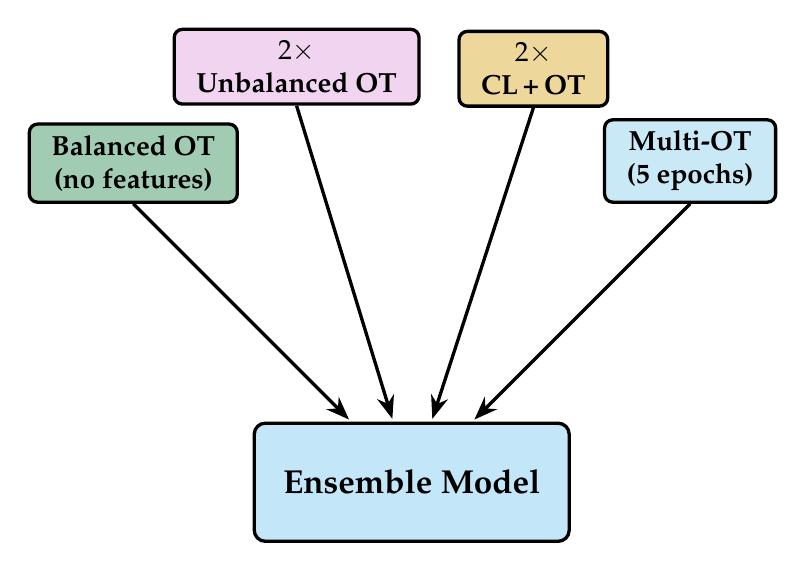
\begin{tikzpicture}[>=Stealth, line width=1.2pt]


\node[draw, fill=Cerulean!25, rounded corners=4pt,
      minimum width=4cm, minimum height=1.5cm,
      font=\large\bfseries, align=center] (ensemble) {Ensemble Model};


\def\radius{5} 

\foreach \idx/\ang/\lab/\col in {
  1/45/{Multi-OT\\(5 epochs)}/SkyBlue!45,
  2/72/{$2\times$\\CL\,+\,OT}/Goldenrod!45,
  3/107/{$2\times$\\Unbalanced OT}/Plum!45,
  4/135/{Balanced OT\\(no features)}/SeaGreen!45
}{
  \node[draw, fill=\col, rounded corners=3pt,
        inner xsep=8pt, inner ysep=4pt,
        font=\bfseries, align=center, anchor=south]
        (M\idx) at (\ang:\radius) {\lab};

  \coordinate (I\idx) at
    (intersection cs:
       first line={(M\idx.south)--(ensemble.center)},
       second line={(ensemble.north west)--(ensemble.north east)});

  \draw[->, shorten >=1pt] (M\idx.south) -- (I\idx);
}

\end{tikzpicture}
\end{document}